\chapter{Proceso de desarrollo de servicio}
\label{capitulocuatro}
%El proceso de desarrollo de servicio web representa la abstracci'on de reutilizaci'on de una aplicaci'on a tr'aves del analisis, los detalles del dise'no, la clasificaci'on del tipo de servicio ofrecido y las etapas de la ingenier'ia de servicio.

%Un componente de software de reutilizaci'on, debidamente ajustado, que ofrece  funcionalidad, se  distribuye y se accede de manera
%program'atica. Un servicio Web es un servicio al que se accede mediante protocolo est'andar de Internet y en XML\footnote{Lenguaje de Marcado Extensible}.
%aumentado por mi
%La revoluci'on del software y el desarrollo de la web en la d'ecada de 1990 mejoro el intercambio de informaci'on entre organizaciones. Las computadoras p'odian obtener informaci'on de organizaciones externas. Es por lo c'ual se propuso la noci'on de servicios web con el objetivo  de apoyar en el intercambio de informaci'on entre organizaciones.
El desarrollo de software y la web en los a'nos de 1990 mejoro el intercambio de informaci'on entre las organizaciones. A traves del proceso de desarrollo de servicios web con el fin de apoyar en el intercambio de informaci'on entre las organizaciones.
\section{El servicio web como componente de reutilizaci'on}
Seg'un Somerville " los servicio web son un desarrollo natural de los componentes de software. Una diferencia fundamental entre un servicio y un componente de software, es que el servicio debe ser independiente y opera en la misma forma, sin importar su entorno de ejecuci'on."\hfill \break
Este servicio web define lo que necesita de otro servicio al establecer sus requerimientos en un mensaje y al enviar el mensaje con la especificaci'on y los detalles de su interfaz. Los cuales se explican a continuaci'on en los documentos de lenguaje de descripci'on de servicios web como WSDL\footnote{WSDL-Lenguaje de descripci'on de servicios web} \cite{Somerville2011}. 
\begin{itemize}
\item En el documento de interface se define las operaciones que soportan el servicio y el formato de los mensajes que env'ian y reciben por parte del mismo servicio.
\item En el documento de enlace mapea la interfaz abstracta a tr'aves de un conjunto concreto de protocolos y especifica los detalles t'ecnicos de c'omo comunicarse con el servicio.
\item En el documento de ubicaci'on se describe la ubicaci'on de la implementaci'on del servicio web en su punto final.
\end{itemize}
El desarrollo de WSDL expresa el servicio web en el formato XML.
\section{La ingenier'ia de servicio}
%Esto es parafraseo
La ingenieria de servicio web es el proceso de desarrollo de servicios para la reutilizaci'on en aplicaciones orientadas a servicios. La ingenier'ia de servicio garantiza que el servicio represente la abstracci'on y la reutilizaci'on, los cuales son 'utiles para otros sistemas. \cite{Somerville2011}. 

Seg'un Somerville exiten tres etapas l'ogicas en el proceso de ingenier'ia de servicio, el c'ual se representa a continuaci'on en la figura \ref{DiagramaIngenieria} y la descripci'on de cada etapa. 
\begin{figure}[H]
\centering
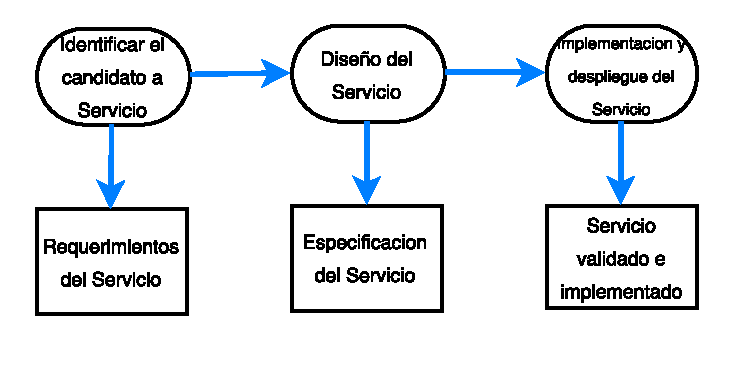
\includegraphics[width=0.6\textwidth]{DiagramaIS.pdf}
\captionsetup{justification=centering,margin=2cm}
\caption{El proceso de ingenier'ia de servicio, adoptado para la realizac'ion del proyecto. El proceso de ingenier'ia de servicio \cite{Somerville2011}}
\label{DiagramaIngenieria}
\end{figure}
La descripci'on de cada etapa l'ogica se explica en las siguientes etapas: 
\begin{itemize}
\item \textbf{Identificaci'on de candidatos a servicios:} la identificaci'on orientada a servicio implica comprender y analizar los procesos empresariales de la organizaci'on para decidir cu'ales servicios de reutilizaci'on podr'ian implementarse. Existen tres tipos de servicios para identificar el servicio los cuales son: servicio utilitario, servicio empresarial y servicio de coordinaci'on o proceso.
El presente proyecto es tipo empresarial porque se trata de servicios asociados con una funci'on empresarial especifica. Para verificar si el servicio es 'util, se plantean las siguientes preguntas las cuales son:\\
\textbf{El cuestionario:} ayuda a reconocer el servicio y verificar el servicio.
\begin{enumerate}
\item ?` El servicio de entidades esta asociado a una entidad l'ogica que se utiliza en diferentes procesos empresariales?
\item ?` Que operaciones soporta la entidad ?
\item ?` Se trata de tareas que realizan diferentes personas en la organizaci'on?
\item ?` El servicio es independiente?
\item ?` El servicio tiene estado?
\item ?` El servicio pueden usar el cliente fuera de la organizaci'on?
\item ?` Diferentes usuarios tienen diferentes requerimientos?
\end{enumerate}
Las respuestas  ayudan a seleccionar y refinar abstracciones para implementar el servicio.
El resultado del proceso de selecci'on de servicios es un conjunto de servicios identificados y requerimientos funcionales del servicio, el cual define que debe hacer el servicio.
\item \textbf{Dise'no de interfaces del servicio:} el dise'no de interface define las operaciones asociadas con el servicio y sus par'ametros. Existen tres etapas en el dise'no de la interfaz del servicio:
\begin{itemize}
\item En el dise'no de interfaz l'ogica comienza con los requerimientos del servicio y define los nombres, par'ametros  de entrada salida, de operaci'on y excepciones.
\item En el dise'no de mensajes se define la estructura de los mensajes que env'ian y reciben el servicio.
\item Desarrollo de WSDL es el dise'no l'ogico y de mensajes se traducen a una descripci'on de interfaz abstracta como se explica anteriormente el documento de interface, el documento de enlace y el documento de ubicaci'on.
\end{itemize}

\item \textbf{Implementaci'on y despliegue del servicio:} una vez concluido los candidatos y los dise'nos de interfaces, la etapa final del proceso de ingenier'ia de servicios es la implementaci'on del servicio. 
\end{itemize}
%aquiiii
\section{Servicios de sistemas heredados}
Seg'un Somerville " los sistemas heredados son sistemas de software antiguos que emplea una organizaci'on, en lo general dependen de tecnolog'ia obsoleta, pero son esenciales para la empresa." Los servicios que se desarrollan para acceder al sistema heredado son coherentes y soportan una sola 'area de su funcionalidad, los cuales se pueden representar graficamente en un diagrama de UML\footnote{UML- Unidad de Lenguaje Modificado}.\cite{Somerville2011}

\section{Desarrollo de software con servicios}
Seg'un Somerville el " desarrollo de software utiliza el  servicio, el c'ual se basan en la idea de que usted combina y configura servicios para crear nuevos servicios compuestos. Estos pueden integrarse con una interfaz de usuario implementada en un navegador para crear una aplicaci'on web".\\
El desarrollo de software con servicios es el proceso de dise'nar nuevos servicios  reutilizando los servicios existente.\\
Seg'un Somerville en la siguiente figura se muestra las etapas de construcci'on de servicio mediante composici'on: 

\begin{figure}[H]
\centering
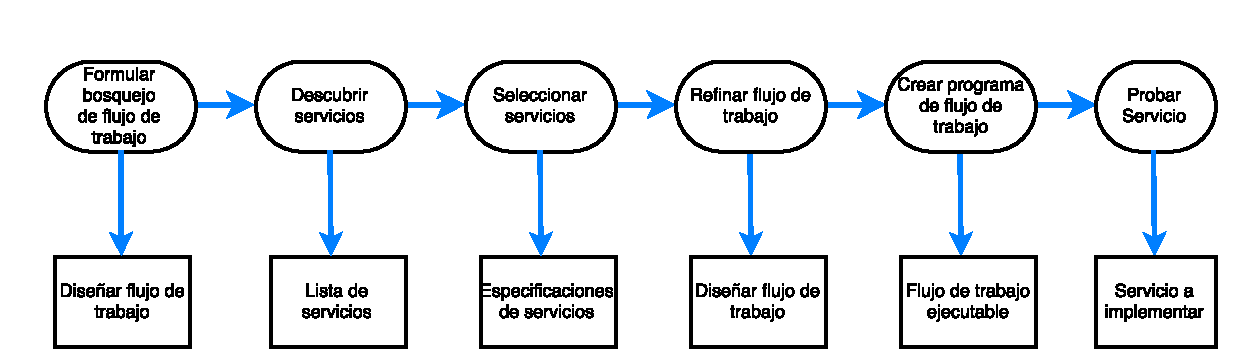
\includegraphics[width=0.8\textwidth]{construirServicio.pdf}
\captionsetup{justification=centering,margin=2cm}
\caption{Etapas de la Construcci'on de servicio, adoptado para la realizac'ion del proyecto. Construci'on de servicio\cite{Somerville2011}}
\label{fig:construccion}
\end{figure}

\begin{itemize}
\item \textit{Formular un bosquejo de flujo de trabajo} comienza con los requerimientos para crear un servicio compuesto, el c'ual es la base para un nuevo dise'no.
\item \textit{El descubrimiento del servicio} se buscan los registros o catalogos de los servicios para descubrir cuales servicio existen, qui'en los proporciona y los detalles de la provisi'on del servicio.
\item \textit{Seleccionar posibles servicios} a partir del conjunto de posibles candidatos a servicio que se han descubierto se seleccionan los posibles servicios que puedan implementar actividades del flujo de trabajo.
\item \textit{Refinar el flujo de trabajo} sobre la base de la informaci'on acerca de los servicios que se selecciona y  se refine el flujo de trabajo.
\item \textit{Crear un programa de flujo de trabajo} durante la etapa el dise'no de flujo de trabajo abstracto se transforma en un programa ejecutable.
\item \textit{Prueba de servicio o aplicaci'on terminada} es el proceso de probar el servicio terminado para realizar la prueba se utilizan los servicios externos.
\end{itemize}
Para concluir se explica el dise'no y las pruebas del flujo de trabajo. Uno de los problemas es la  reutilizaci'on dentro de la organizaci'on.


\subsection{Dise'no e implementaci'on del flujo de trabajo} 
Seg'un Somerville " dise'no de flujo de trabajo implica analizar los procesos empresariales existentes o planeados para comprender las diferentes actividades que se realizan, estas intercambian informaci'on, luego se define el nuevo proceso empresarial en la notaci'on de flujo de trabajo".  
Si los procesos empresariales tienen  diferentes partes de una organizaci'on estas se pueden separar mediante carriles. 
Una vez concluido con el dise'no final, el c'ual se debe convertirse en un programa ejecutable. \cite{Somerville2011}
\begin{itemize}
\item \textit{Implementar los servicios} se debe tener en cuenta que los servicios son independientes del lenguaje de implementaci'on.
\item \textit{Generar una versi'on ejecutable} del modelo de flujo de trabajo traducirlo a un c'odigo de manera manual o automatica.
\end{itemize}
\subsection{Pruebas del servicio} 
Las pruebas son importantes para los procesos de desarrollo de sistemas, estos muestran que un sistema cumple con los requerimientos funcionales y detectan defectos introducidos durante el proceso de desarrollo.\cite{Somerville2011} 

Seg'un Somerville " para comprender la implementaci'on del servicio se debe presentar dificultades cuando se prueba el servicio y la combinaci'on de los servicios". 

Seg'un Somerville a continuaci'on los tipos de prueba del servicio.
\begin{enumerate}
\item \textit{Prueba de servicio o aplicaci'on terminada} es el proceso de probar el servicio terminado, es complejo cuando se usa servicios externos.
\item \textit{Los servicios externos} est'an bajo el control de proveedor de servicio y no del usuario del servicio. El proveedor puede retirar los servicios, dicho problema se debe manejar como componentes para mantener las versiones.
\item \textit{Los servicios a largo plazo} la aplicaci'on puede usar otro servicio.
\item \textit{El comportamiento no funcional} no depende solo de como se usa, por parte de la aplicaci'on que se pone a prueba.
\item \textit{El modelo de pago} para los servicios se puede hacer que los servicios sean muy costosos. Se debe utilizar servicios que son gratuitos. 
\end{enumerate}
%debemos unir estas dos figuras que cumpla con la estructura q he definido
%Para el proceso de construcci'on  de servicio mediante composici'on, se muestran 6 etapas en la figura  \ref{fig:construccion}:

%\begin{figure}[H]
%\centering
%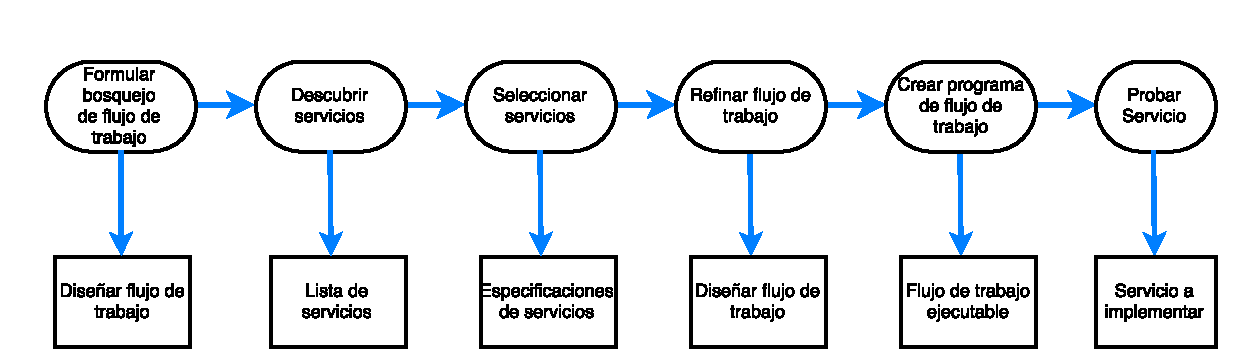
\includegraphics[width=0.8\textwidth]{construirServicio.pdf}
%\captionsetup{justification=centering,margin=2cm}
%\caption{Etapas de la Construcci'on de servicio, adoptado para la realizac'ion del proyecto. Construci'on de servicio\cite{Sommerville2012}}
%\label{fig:construccion}
%\end{figure}
%A continuaci'on se explica cada etapa de la figura  \ref{DiagramaIngenieria} de la ingenier'ia de servicio.


%\section{Tipos de servicio web}
%Se tiene 3 tipos de servicios son: utilitarios, empresariales y coordinaci'on o proceso.Para el presente proyecto, se ha definido un servicio empresarial, que se explica a continuaci'on.

%\begin{itemize}
%\item \textbf{Servicio empresarial,} se trata de servicios asociados, con una funci'on empresarial especifica. Un ejemplo de una funci'on empresarial es una universidad ser'ia la inscripci'on de estudiantes para un curso u otros. 
%\end{itemize}


%\section{Identificar los candidatos a servicio}
%Para identificar el candidato a servicio se debe comprender y analizar los procesos empresariales de la organizaci'on. Los procesos empresariales aportan en la identificaci'on del servicio y desde los procesos se determinan el servicio a ser reutilizado. Este servicio debe ser l'ogicamente coherente, independiente y reutilizado por lo c'ual puede ser orientados a entidades o tareas y estas son asociadas con alguna actividad.
%Para verificar  el candidato al servicio se debe plantear el cuestionario, el proceso de selecci'on y el flujo de trabajo. A continucaci'on se explican el cuestionario, el proceso de selecci'on y el flujo de trabajo.

%\begin{itemize}
%\item \textbf{El cuestionario:} ayuda a reconocer el servicio y verificar si el servicio es 'util. A continuaci'on las preguntas del cuestionario.
%\begin{enumerate}
%\item �El servicio de entidades esta asociado a una entidad l'ogica que se utiliza en diferentes procesos empresariales?
%\item �Que operaciones soporta la entidad ?
%\item �Se trata de tareas que realizan diferentes personas en la organizaci'on?
%\item �El servicio es independiente?
%\item �El servicio tiene estado?
%\item �El servicio pueden usar el cliente fuera de la organizaci'on?
%\item �Diferentes usuarios tienen diferentes requerimientos?
%\end{enumerate}
%Despues de terminar el cuestionario se analiza las respuestas, para comenzar analizar el proceso de selecci'on.
%\item \textbf{Proceso de selecci'on:} es un conjunto de actividades orientadas para realizar parte del trabajo con el fin de alcanzar una meta de los servicios identificados, el c'ual  tiene 6 etapas claves de proceso de construcci'on las cuales se explican a continuaci'on:

%\begin{enumerate}
%\item Formular el bosquejo de flujo de trabajo se usan los requerimientos para el servicio compuesto con el fin de conocer los servicios disponibles.
%\item Descubrimiento de servicios se buscan los servicios existente, qui'en los  proporciona y los detalles.
%\item Seleccionar posibles servicios a partir de los candidatos a servicios y teniendo en cuenta los criterios de selecci'on incluir'an  las funcionalidades de los servicios ofrecidos.
%\item Refinar el flujo de trabajo sobre la base de la informaci'on acerca de servicio que se han seleccionado se refina el flujo de trabajo. Se vuelve a repetir la etapa de descubrimiento y selecci'on. 
%\end{enumerate}

%inicio de aumentado
%\item \textbf {Dise'no de Flujo de trabajo}
%Es el conjunto de actividades orientadas para realizar parte del trabajo, el c'ual establece los pasos necesarios para alcanzar Los detalles del flujo de trabajo ayudan a organizar las actividades del servicio web las cuales son:
%\begin{enumerate}
%\item \textbf{Flujo de trabajo,} es un conjunto de actividades orientadas para realizar parte del trabajo, el c'ual establece los pasos necesarios para alcanzar una meta particular.
%El dise'no de flujo de trabajo analiza los procesos planeados, al comprender las actividades, al realizar el intercambio de informaci'on, para definir las etapas de proceso.
%El flujo de trabajo se representa en el diagrama de actividades de UML\footnote{Unidad de Lenguaje Modificado}.
%Tiene algunos conceptos centrales de BPMN\footnote{Proceso de Negocio de Modelo de Notaci'on}, se utiliza para crear el modelo de flujo de trabajo.  A continuaci'on se explica los detalles del flujo de trabajo.
%\begin{itemize}
%\item La actividad se representan mediante un rect'angulo con esquinas redondeadas. Una actividad puede ejecutarse por una persona o por un servicio automatizado.
%\item El evento se representa en c'irculo. Un evento es algo que sucede durante un proceso: evento inicial(c'irculo claro), evento final(c'irculo oscuro), evento intermedio (c'irculo doble no se muestra) se ejecuta peri'odicamente.
%\item Las compuertas se representa mediante un diamante, es una etapa en el proceso para utilizar una elecci'on.
%\item La secuencia de actividades, se representa mediante una flecha s'olida, se usa para mostrar la secuencia de actividades. El mensaje que fluyen entre actividades se representan en una flecha punteada.
%\end{enumerate}
%\end{itemize}
%\item \textbf{Acci'on de compensaci'on}
%La acci'on de compensaci'on se utiliza para deshacer acciones, que se completan, el c'ual deben cambiar el resultado de posteriores actividades del flujo de trabajo.
%\end{enumerate}


%fin de aumentado

%\section{El dise'no de servicio web}
%Una vez concluida, con  la identificaci'on del servicio, se realiza las operaciones asociadas con el servicio y sus p'arametros, el dise'no de operaciones y los mensajes de servicio. El dise'no se representa en 3 tipos, para el presente proyecto se utiliza los siguientes: 
%\begin{enumerate}
%\item Dise'no de interfaz l'ogica, se identifica las operaciones asociadas con el servicio, sus entradas y salidas, as'i como las excepciones asociadas con dichas operaciones. Despu'es se realiza los requerimientos del servicio, define los nombres y par'ametros de operaci'on. Se debe definir las excepciones que s'urgen cuando se ubica una operaci'on de servicio.
%\item Dise'no de mensajes, es la estructura de los mensajes que env'ia y recibe el servicio. Define los mensajes de entrada y salida, el manejo de mensajes como objetos, la estructura en operaci'on y excepciones.
%\end{enumerate}

%Una vez concluido, con el dise'no para an'alisis del servicio, se realiza el dise'no para desarrollar el servicio con flujo de trabajo.

%\begin{enumerate}
%\item \textbf{Crear un programa de flujo de trabajo,} es  el dise'no de flujo de trabajo, para transformar en un programa ejecutable.
%\item \textbf{Crear un dise'no de datos de servicio,} es el dise'no para mostrar el formato de informaci'on, para utilizar el servicio web. 
%\end{enumerate}


%\section{Implementaci'on del servicio web}

%El modelo puede realizar algunas iteraciones, hasta que se cree un dise'no que permite la reutilizaci'on de los servicios disponibles.
%Utilizamos el dise'no de desarrollo del servicio de flujo de trabajo, que se debe convertira en un programa ejecutable, esto implica la actividad de:
%\begin{enumerate}
%\item Implementar los servicios, los servicios son independientes del lenguaje de implementaci'on, dichos servicios se pueden escribir en cualquier lenguaje de programaci'on.
%\end{enumerate}

%\section{Pruebas del servicio}
%Las pruebas son importante en todos los procesos de desarrollo del sistema se muestran que un sistema cumple con los requerimientos funcionales cuando se utiliza un servicio externo 'esto significa que no se tiene acceso a su co'digo fuente es por lo c'ual que no se debe hacer en base a c'odigo fuente.
%Para comprender lo implementaci'on se debe realizar prueba y combinaci'on de los servicios:
%\begin{itemize}
%\item \textbf{Prueba de servicio o aplicaci'on terminada,} es el proceso de probar el servicio terminado, es complejo cuando se usa servicios externos.
%\item \textbf{Los servicios externos,} est'an bajo el control de proveedor de servicio y no del usuario del servicio. El proveedor puede retirar los servicios, dicho problema se debe manejar como componentes para mantener las versiones.
%\item \textbf{Los servicios a largo plazo,} la aplicaci'on puede usar otro servicio.
%\item \textbf{El comportamiento no funcional,} no depende solo de como se usa, por parte de la aplicaci'on que se pone a prueba.
%\item \textbf{El modelo de pago,} para los servicios se puede hacer que los servicios sean muy costosos. Se debe utilizar servicios que son gratuitos. 
%\end{itemize}

\section{El dise'no metodolog'ico}
El dise'no metodolog'ico para el presente proyecto se realizo en base a la puntos anteriores teniendo como resultado la siguiente figura \ref{fig:Diagrama} que representa la secuencia de procesos de desarrollo para este proyecto.

\begin{figure}[H]
\centering
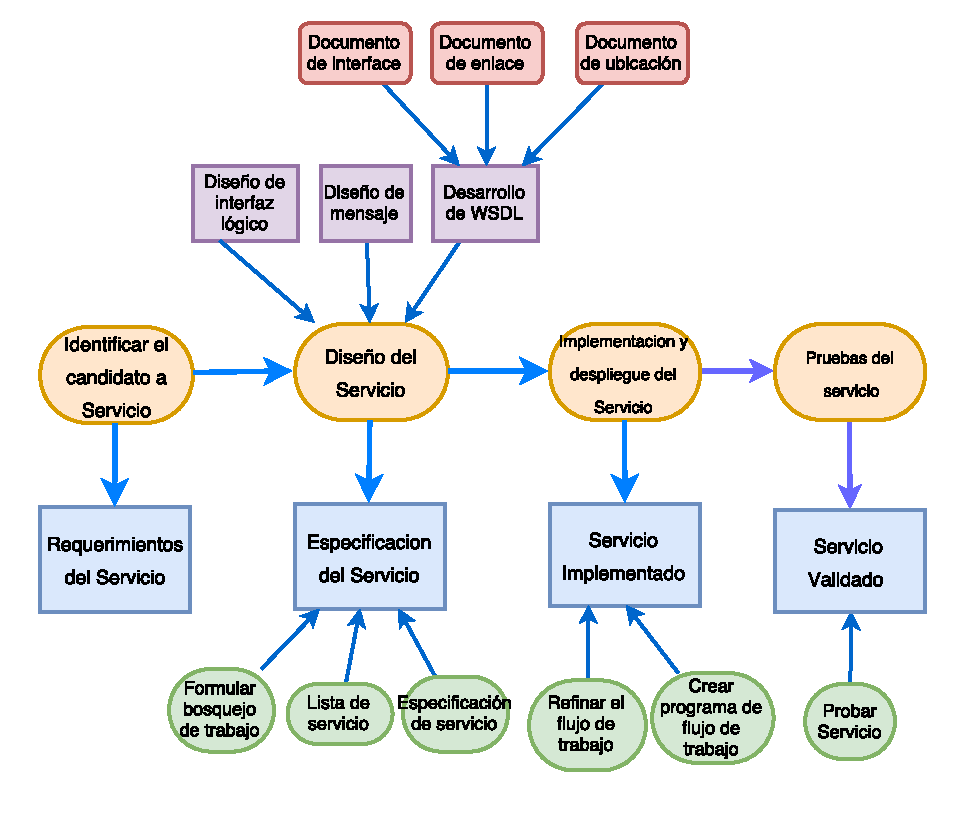
\includegraphics[width=0.7\textwidth]{DiagramaDServicio.pdf}
\captionsetup{justification=centering, margin=2cm}
\caption{Secuencia de pasos para el proceso de ingeniera. Fuente: En base a la construcci'on de servicio de Somerville \cite{Somerville2011}}
\label{fig:Diagrama}
\end{figure}

El presente proyecto es un sistemas heredado porque utiliza como antecedente a la p'agina del SAGAA para el desarrollo del servicio web. Es por lo c'ual se ha incorporado las etapas de construcci'on de servicio mediante composici'on  en el modelo metodol'ogico.

\section{Conclusiones}
La arquitectura de servicios web utiliza el desarrollo de componentes como base para la etapa de construcci'on del servicio web.

Los sistemas heredados utilizan un servicio web existente de una organizaci'on para crear un nuevo servicio web con la herramienta de diagrama de flujos de trabajo.

El dise'no metodol'ogico utiliza el dise'no de servicio como base y complementa con la herramienta del desarrollo de software de servicio por componentes para la etapa de dise'no del servicio con los diagrama de flujos.

%En el cap'itulo \ref{capitulocuatro} se explicar'a el proceso de ingenier'ia de software del SOA y en el c'apitulo \ref{capitulodos}, se explican las herramientas para cumplir con el objetivos de \textit{Proveer servicio web de la p'agina del SAGAAA} \ref{sec:oe} en el presente proyecto.\\

%En el cap'itulo \ref{capitulotres} se explica los detalles y procesos para cumplir con el objetivo 1 y la recolecci'on de datos.\\

%En el c'apitulo \ref{capitulocinco} se explica el  analisis, dise'no e implementaci'on del servicio web, como se muestra en la figura \ref{fig:Diagrama} en el n'umero 1 - 3 para cumplir con el objetivo 4.\\
 
%En el c'apitulo \ref{capituloseis}, se explica el analisis y dise'no de la aplicaci'on m'ovil, como se muestra en la figura \ref{fig:Diagrama} en el n'umero 4, para cumplir con el objetivo 4 y en parte al objetivo 1 del c'ual se tiene a continuaci'on el c'apitulo \ref{capitulosiete}, en donde se realiza la implementaci'on de la aplicaci'on m'ovil, como se muestra en la figura \ref{fig:Diagrama} en el n'umero 5 cumpliendo con el objetivo 1 y 3.\\
%En el c'apitulo \ref{capitulonueve} se trata de la prueba de la aplicac'ion m'ovil y el servicio web, como se muestra en la figura \ref{fig:Diagrama} en el n'umero 6, para cumplir con el objetivo general \ref{og} de proveer el servicio del SAGAA, a tr'aves de una aplicaci'on m'ovil.\\

%En el c'apitulo \ref{capituloocho} es el dise'no adaptativo de la aplicaci'on m'ovil que responde al objetivo 2.

%Para el desarrollo de la metodologia se utiliza las siguentes plataformas de desarrollo, se explican a continuaci'on.